\documentclass[tikz,border=8pt]{standalone}
\usepackage{tikz}
\usetikzlibrary{arrows.meta,calc}
\begin{document}
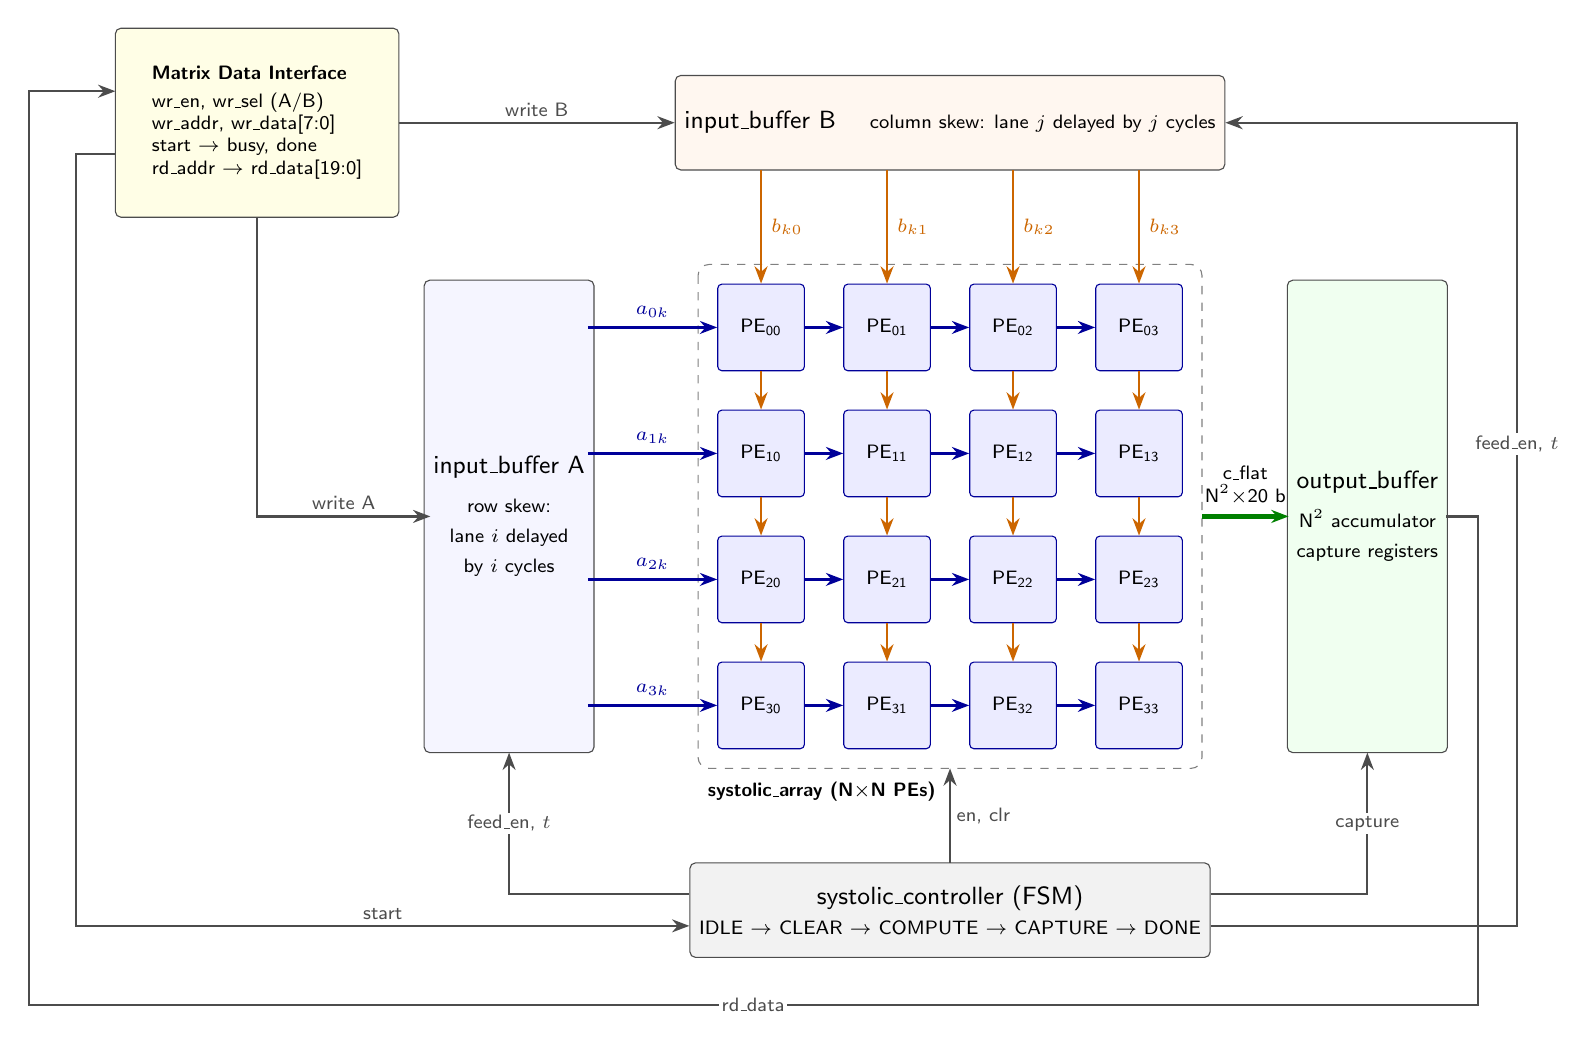
\begin{tikzpicture}[
  font=\sffamily\small, >={Stealth[length=2.2mm]},
  blk/.style={draw=black!70, rounded corners=2pt, fill=#1, align=center},
  pe/.style={draw=blue!60!black, fill=blue!8, minimum size=11mm, rounded corners=1.5pt, font=\sffamily\scriptsize},
  lbl/.style={font=\sffamily\scriptsize, fill=white, inner sep=1pt},
  bus/.style={->, thick, black!70}, hbus/.style={->, thick, blue!60!black},
  vbus/.style={->, thick, orange!80!black}]

% ---------------- PE grid ----------------
\foreach \i in {0,...,3}{\foreach \j in {0,...,3}{
  \node[pe] (p\i\j) at (\j*1.6, -\i*1.6) {PE\textsubscript{\i\j}};}}
\foreach \i in {0,...,3}{\foreach \j/\k in {0/1,1/2,2/3}{\draw[hbus] (p\i\j) -- (p\i\k);}}
\foreach \j in {0,...,3}{\foreach \i/\k in {0/1,1/2,2/3}{\draw[vbus] (p\i\j) -- (p\k\j);}}
\draw[black!50, dashed, rounded corners] (-0.8,0.8) rectangle (5.6,-5.6);
\node[font=\sffamily\scriptsize\bfseries, anchor=north west] at (-0.8,-5.65) {systolic\_array (N$\times$N PEs)};

% ---------------- A input buffer (left) ----------------
\node[blk=blue!4, minimum width=20mm, minimum height=60mm] (abuf) at (-3.2,-2.4)
  {input\_buffer A\\[3pt]\scriptsize row skew:\\\scriptsize lane $i$ delayed\\\scriptsize by $i$ cycles};
\foreach \i in {0,...,3}{\draw[hbus] (-2.2,-\i*1.6) -- node[above,font=\scriptsize]{$a_{\i k}$} (p\i0.west);}

% ---------------- B input buffer (top) ----------------
\node[blk=orange!6, minimum width=60mm, minimum height=12mm] (bbuf) at (2.4,2.6)
  {input\_buffer B \quad\scriptsize column skew: lane $j$ delayed by $j$ cycles};
\foreach \j in {0,...,3}{\draw[vbus] (\j*1.6,2.0) -- node[right,font=\scriptsize]{$b_{k\j}$} (p0\j.north);}

% ---------------- output buffer (right) ----------------
\node[blk=green!6, minimum width=20mm, minimum height=60mm] (obuf) at (7.7,-2.4)
  {output\_buffer\\[3pt]\scriptsize N$^2$ accumulator\\\scriptsize capture registers};
\draw[->, line width=2pt, green!50!black] (5.6,-2.4) -- node[above,font=\sffamily\scriptsize,align=center,text=black]{c\_flat\\N$^2{\times}$20 b} (6.7,-2.4);

% ---------------- controller (bottom) ----------------
\node[blk=gray!10, minimum width=60mm, minimum height=12mm] (ctrl) at (2.4,-7.4)
  {systolic\_controller (FSM)\\\scriptsize IDLE $\to$ CLEAR $\to$ COMPUTE $\to$ CAPTURE $\to$ DONE};
\draw[bus] (2.4,-6.8) -- node[lbl,right=1pt]{en, clr} (2.4,-5.6);
\draw[bus] ([yshift=2mm]ctrl.west) -| node[lbl,pos=0.75]{feed\_en, $t$} (-3.2,-5.4);
\draw[bus] ([yshift=2mm]ctrl.east) -| node[lbl,pos=0.75]{capture} (7.7,-5.4);
\draw[bus] ([yshift=-2mm]ctrl.east) -| node[lbl,pos=0.8]{feed\_en, $t$} (9.6,2.6) -- (bbuf.east);

% ---------------- host / matrix data interface ----------------
\node[blk=yellow!10, minimum width=36mm, minimum height=24mm, align=left, font=\sffamily\scriptsize] (host) at (-6.4,2.6)
  {\textbf{Matrix Data Interface}\\[2pt]wr\_en, wr\_sel (A/B)\\wr\_addr, wr\_data[7:0]\\start $\to$ busy, done\\rd\_addr $\to$ rd\_data[19:0]};
\draw[bus] (-4.6,2.6) -- node[lbl,above=1pt]{write B} (bbuf.west);
\draw[bus] (-6.4,1.4) |- node[lbl,pos=0.75,above=1pt]{write A} (-4.2,-2.4);
\draw[bus] (-8.2,2.2) -- (-8.7,2.2) |- node[lbl,pos=0.75,above=1pt]{start} ([yshift=-2mm]ctrl.west);
\draw[bus] (8.7,-2.4) -- (9.1,-2.4) -- (9.1,-8.6) -- node[lbl,pos=0.5]{rd\_data} (-9.3,-8.6) |- (-8.2,3.0);
\end{tikzpicture}
\end{document}
